\documentclass[border=3mm,tikz]{standalone}
\usepackage{pgfplots}

\pgfplotsset{compat=1.10}
\usepgfplotslibrary{fillbetween}
\usetikzlibrary{patterns}

\begin{document}

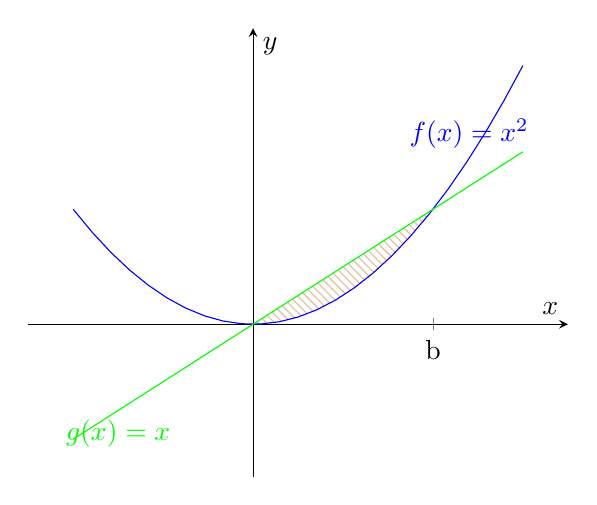
\begin{tikzpicture}
\begin{axis}[axis lines=middle,
            xlabel=$x$,
            ylabel=$y$,
            enlargelimits,
            ytick=\empty,
            xtick={0,1},
            xticklabels={a,b}]
\addplot[name path=F,blue,domain={-1:1.5}] {x^2} node[pos=.8, above]{$f(x)=x^2$};

\addplot[name path=G,green,domain={-1:1.5}] {x}node[pos=.1, below]{$g(x)=x$};

\addplot[pattern=north west lines, pattern color=brown!50]fill between[of=F and G, soft clip={domain=0:1}]
;
\node[coordinate,pin=30:{$A$}] at (axis cs:3.8,3){};

\end{axis}
\end{tikzpicture}


\end{document}
